\graphicspath{ {images/} }


\paragraph{Descrierea scenei si a obiectelor}

\begin{itemize}
\item
	\tab Scena prezentata in aceasta lucrare de laborator este o inspiratie din jocul Wolfenstein \footnote{https://en.wikipedia.org/wiki/Wolfenstein} infaptuita adunand modele si texturi de pe anumite site-uri specifice. \footnote{Pentru anumite modele: www.free3dmodel.com ori www.models.com\\ \tab Pentru texturi : www.textures.com ori google images\\}.\\
	\tab Scena a fost prelucrata in programul Blender , obiectele fiind incarcate in diferite formaturi \footnote{.fbx which is more used in autodesk programs\\\tab .obj ce reprezinta obiecte geometrice, acesta fiind cel mai des utilizat, si fiind formatul suportat predefinit de libraria glm} si avand diferite texturi, in general de calitate superioara (peste 1000pixeli) si respectand formatul de putere al lui 2.(521px, 1024,2048px). Ele au fost mapate pe obiectele din scena folosind maparea UV.\\
	\tab Cateva imagini reprezentative ale proiectului.\\

\begin{center}
  	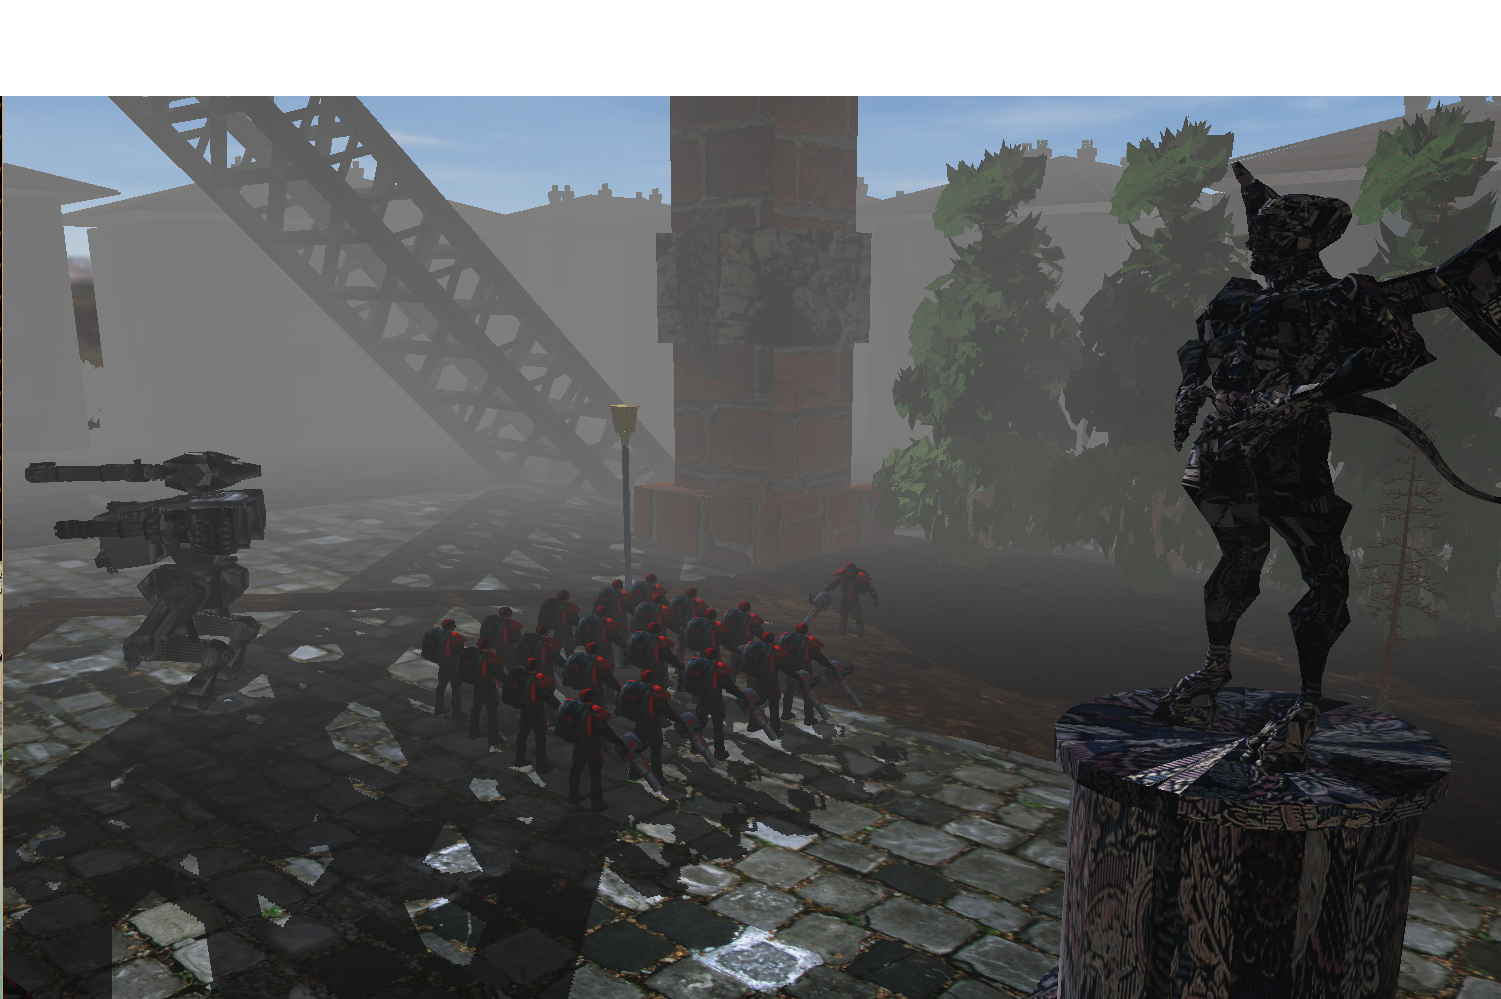
\includegraphics[scale=0.4]{1}
\end{center}

	\tab In mod wireframe arata cam asa. \\
\begin{center}
  	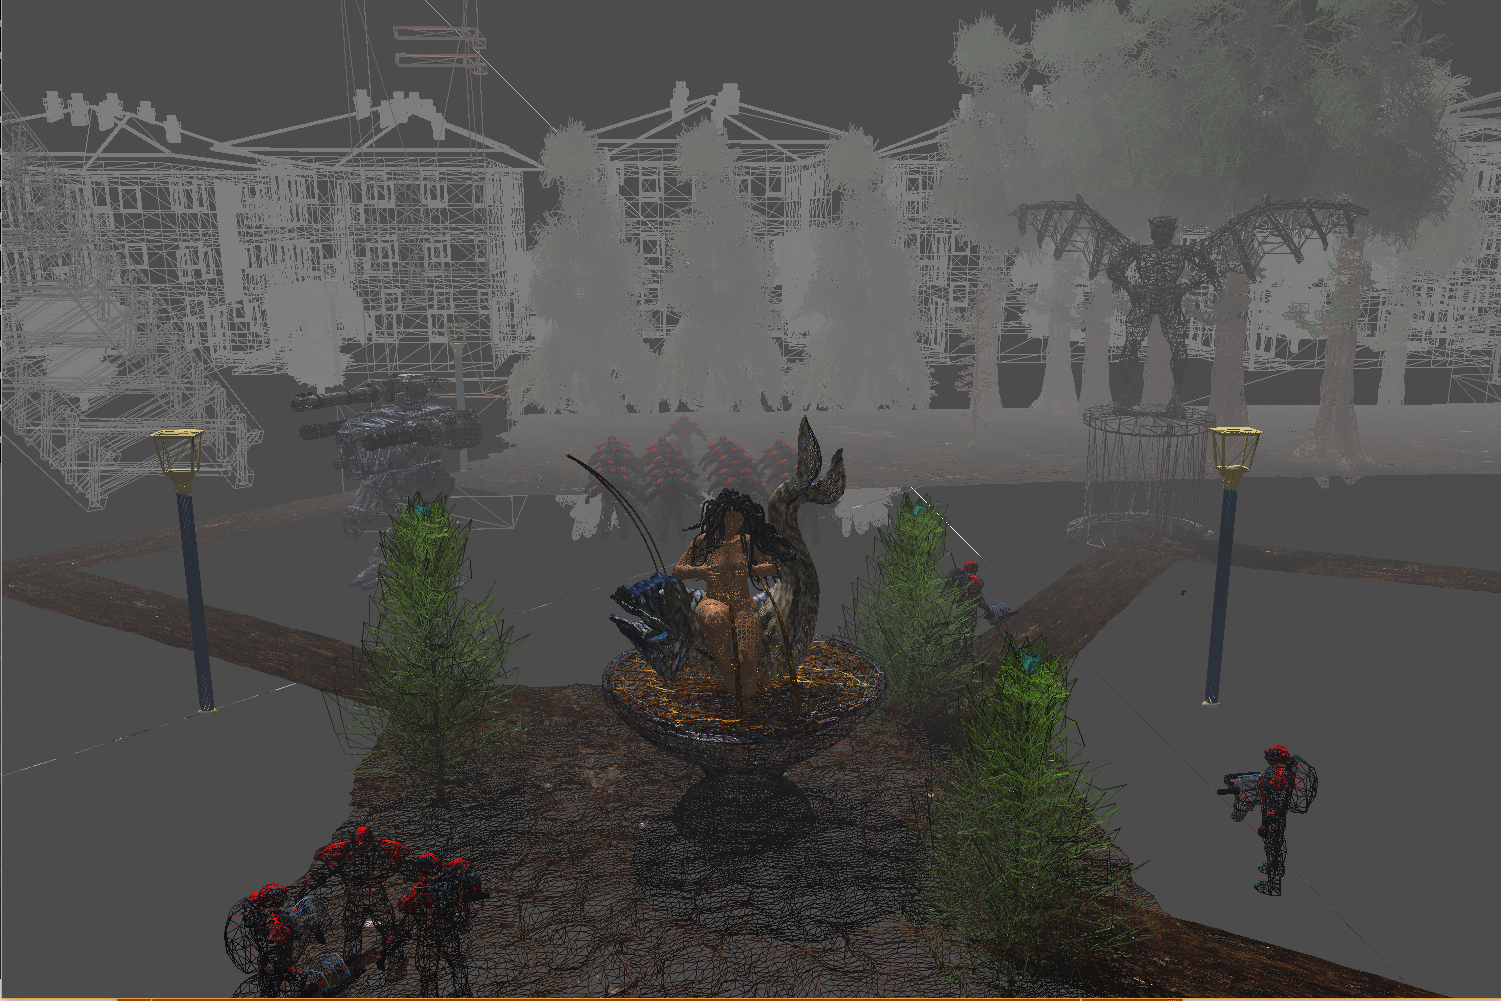
\includegraphics[scale=0.4]{4}
\end{center}

\begin{center}
  	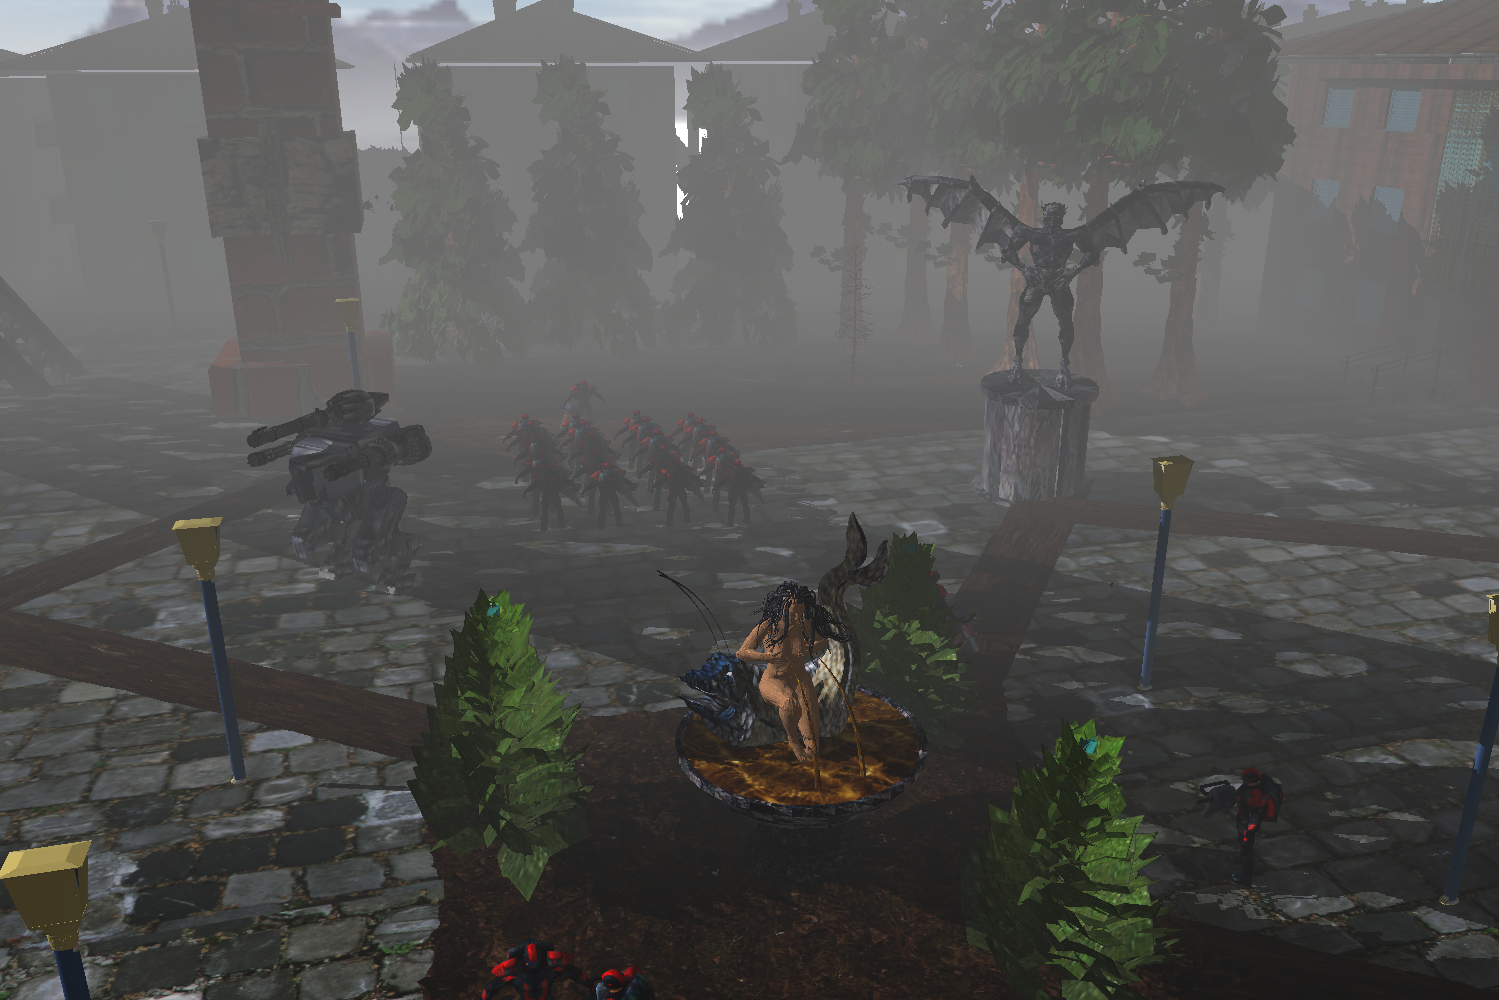
\includegraphics[scale=0.4]{2}
\end{center}

\begin{center}
  	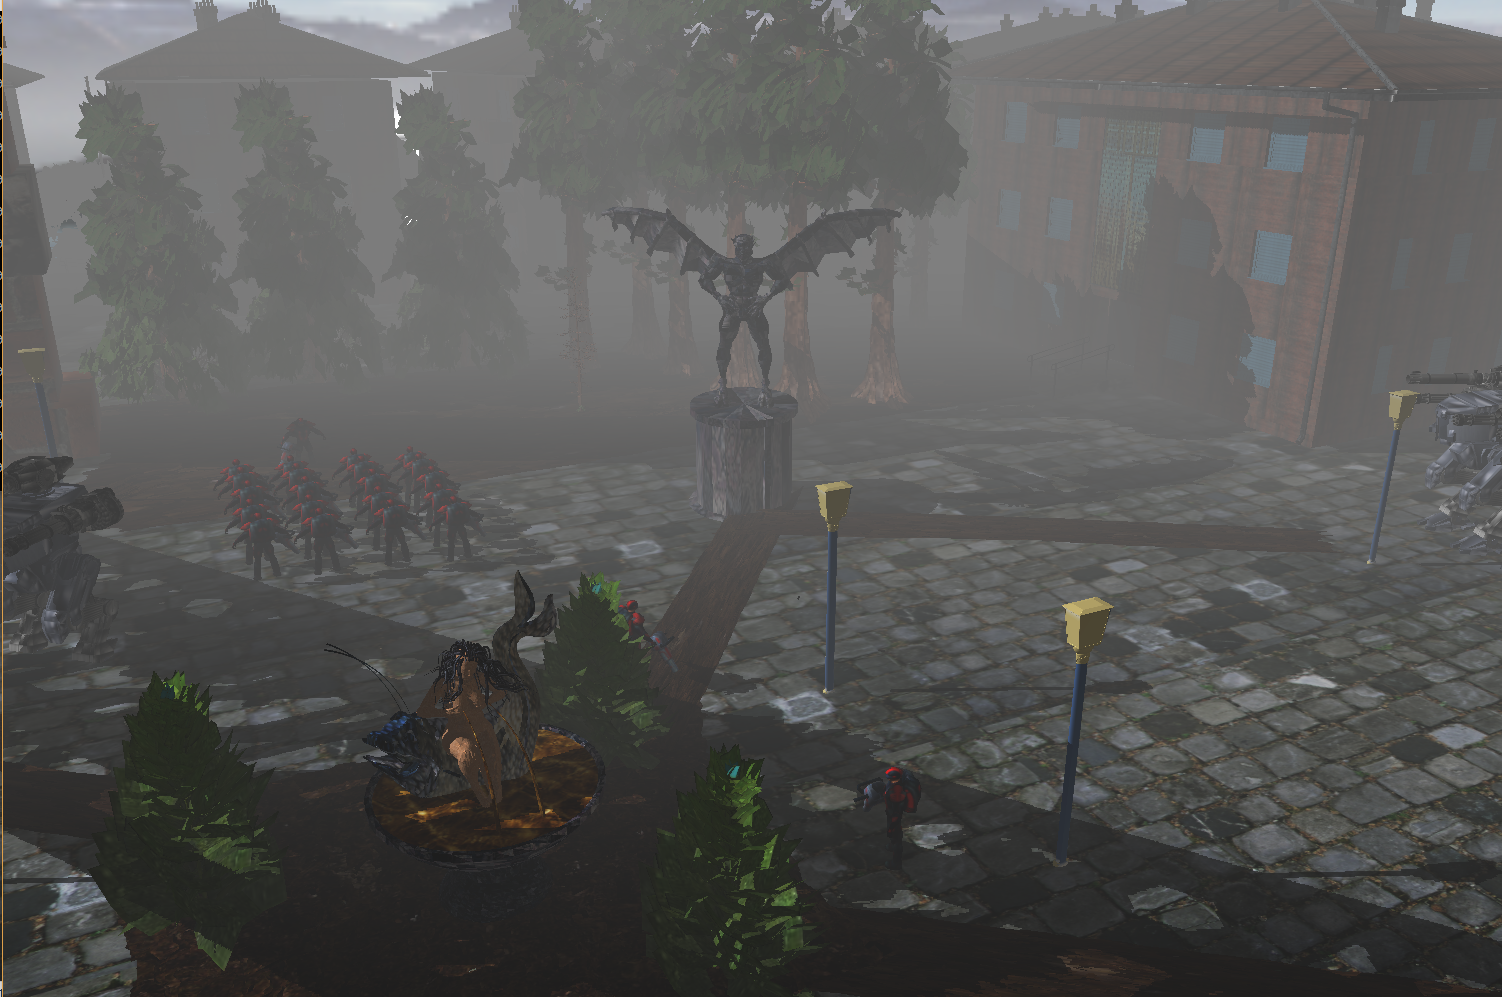
\includegraphics[scale=0.4]{3}
\end{center}

\end{itemize}

\paragraph{ Funcționalități}
\begin{itemize}
\item
	\tab Se poate plimba cu o camera implementata prin scena , se pot vedea ozn-uri pe cer, soldati, case , roboti etc.\\
	\tab Camera la inceput va prezenta o imagine de persepctiva asupra scenei prezentate.\\
\end{itemize}
